% Chapter 3 -- Claim: Size and Value Explain Returns That Beta Cannot (was Ch. 3)
% Figures need tikz and pgfplots (with the fillbetween library) in the preamble.
\providecolor{fenavy}{HTML}{1B2A6B}
\providecolor{fegray}{HTML}{4D4D4D}

\chapter{Claim: Size and Value Explain Returns That Beta Cannot}
\label{ch:03}

The Capital Asset Pricing Model (CAPM) provides a foundational answer to a central question in finance: why should assets with different risk characteristics earn different expected returns? In its standard form, the CAPM predicts that expected excess returns are proportional to market beta. Once beta is taken into account, firm characteristics such as size, valuation ratios, profitability, and investment should not provide additional information about expected returns. This implication makes the model empirically testable: if portfolios with different characteristics continue to earn different average returns after controlling for market exposure, the single-factor model is incomplete.

Early empirical studies found evidence of a positive relation between market beta and average returns, although the strength of that relation was not always consistent with the CAPM's predictions (Black, Jensen, and Scholes 1972; Fama and MacBeth 1973). Later studies documented return patterns associated with firm characteristics. Basu (1977) found that stocks with low price--earnings ratios earned higher returns than the CAPM would predict. Banz (1981) documented a size effect, while Rosenberg, Reid, and Lanstein (1985) reported higher returns for stocks with high book-to-market ratios. These findings raised a basic question: could market beta alone explain the cross-section of average stock returns?

Fama (1970) emphasized that tests of market efficiency are joint tests of market efficiency and the model used to measure expected returns. An apparent return anomaly may therefore indicate either market mispricing or an incomplete asset-pricing model. Fama and French (1992) showed that size and book-to-market equity helped explain differences in average returns that market beta did not adequately explain in their sample. They subsequently developed a three-factor model incorporating the market, size, and value factors (Fama and French 1993). Later work extended this framework by adding profitability and investment (Fama and French 2015). These models became influential tools for describing portfolio returns and evaluating investment performance.

The economic interpretation of these return patterns remains debated. A risk-based interpretation views size and value factors as proxies for common sources of risk for which investors require compensation. A behavioral interpretation argues that some premiums arise because investors extrapolate past growth, overreact to disappointing news, or misprice firms (Lakonishok, Shleifer, and Vishny 1994). The same empirical pattern can therefore be consistent with different explanations. A factor model can describe return differences without, by itself, establishing why those differences exist.

Multifactor models also have practical consequences. They affect how investors distinguish manager skill from exposure to systematic factors, how researchers evaluate fund performance, and how companies estimate the cost of equity (Graham and Harvey 2001). At the same time, the proliferation of proposed factors creates a statistical challenge. Harvey, Liu, and Zhu (2016) catalogued 316 factors across 313 published works and selected working papers, while noting that the number of factors actually tested was likely larger because unsuccessful experiments often remain unpublished. Their analysis argues that newly proposed factors should face a more demanding statistical hurdle than the conventional threshold of approximately 2.

The claim examined in this chapter is therefore: \textbf{size and value factors help explain differences in portfolio returns that the CAPM does not adequately explain, but the search for additional factors creates a multiple-testing problem that requires stronger statistical evidence.}

The chapter develops this argument in three stages. First, it reviews the statistical foundations needed to describe return distributions and interpret linear regressions. Second, it traces the development from the CAPM to the Fama--French three- and five-factor models, considers competing explanations for factor premiums, and examines the factor zoo and the multiple-testing problem. Third, the lab compares the CAPM and the Fama--French three-factor model using the 25 portfolios formed on size and book-to-market, then uses a controlled simulation to illustrate how testing many candidate factors can generate false discoveries.

By the end of the chapter you will be able to:
\begin{itemize}
  \item describe return distributions using the mean, variance, skewness, kurtosis, and autocorrelation, and interpret a basic linear regression;
  \item distinguish systematic risk from idiosyncratic risk and explain the role of beta in the CAPM;
  \item explain how the Fama--French three- and five-factor models extend the CAPM, and interpret alpha and factor loadings;
  \item describe the economic interpretations of size, value, profitability, and investment premiums, including the distinction between risk-based and behavioral explanations;
  \item explain why testing many candidate factors increases the probability of false discoveries;
  \item summarize the main findings of Harvey, Liu, and Zhu (2016), including their recommendation that newly discovered factors generally require a $t$-statistic greater than 3.0;
  \item distinguish statistical significance from economic significance and identify practical considerations that affect the implementation of factor strategies.
\end{itemize}

In the lab, you will estimate the CAPM and the Fama--French three-factor model for the 25 size-and-book-to-market portfolios, compare their explanatory performance, and conduct a simulation in which all candidate factors have known zero premiums.

\section{Foundations: distributions and regression}
\label{sec:03-foundations}

This section reviews two tools used throughout empirical asset pricing: summary statistics for return distributions and linear regression. Readers familiar with these methods may skim the section, but the notation and distinctions introduced here will be useful in the model comparisons that follow.

\subsection{Describing a distribution}
Four commonly used statistical moments summarize important features of a return distribution:
\begin{itemize}
  \item The \textbf{mean}\index{mean} is its center: the average return.
  \item The \textbf{variance}\index{variance|textbf}, or its square root, the standard deviation\index{standard deviation}, measures spread: how far returns typically fall from the mean.
  \item \textbf{Skewness}\index{skewness|textbf} measures asymmetry around the mean. Negative skewness indicates a longer or heavier left tail, so unusually large losses are more prominent than unusually large gains.
  \item \textbf{Kurtosis}\index{kurtosis|textbf} measures the weight of a distribution's tails relative to a normal distribution. A normal distribution has kurtosis 3; a value above 3 implies positive excess kurtosis and indicates greater weight in the tails.
\end{itemize}

Figure~\ref{fig:03-moments} illustrates how each moment changes the shape of a distribution. The mean and variance describe its center and spread, while skewness and kurtosis describe features that a mean--variance summary can miss. Two portfolios can have the same average return and standard deviation but very different probabilities of extreme losses.

\begin{figure}[htbp]
\centering
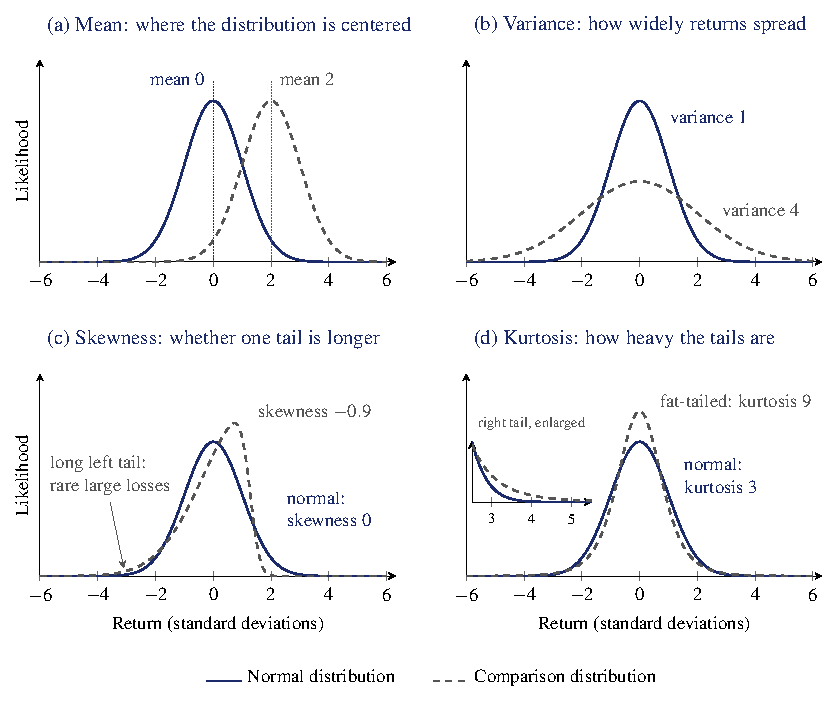
\includegraphics[width=0.7\linewidth]{images/fig03-0-moments.pdf}
\caption{The four moments of a distribution. Each panel compares the standard normal distribution (solid) with one that differs in a single respect. (a)~The mean sets the center. (b)~The variance sets the spread. (c)~Negative skewness lengthens the left tail, so large losses are more likely than large gains of the same size. (d)~Higher kurtosis puts more weight in the tails: the normal distribution has kurtosis 3, the fat-tailed one shown has kurtosis 9. Panels (c) and (d) keep the mean and variance of the normal distribution.}
\label{fig:03-moments}
\end{figure}

A fifth measure describes dependence over time. \textbf{Autocorrelation}\index{autocorrelation|textbf} is the correlation between a series and its own lagged values. The first-order autocorrelation ($\rho_1$) compares each month's return with the previous month's return. A value near $+1$ indicates strong positive linear dependence; a value near $-1$ indicates strong negative linear dependence; and a value near zero indicates little linear dependence at that lag. Zero autocorrelation does not rule out every form of predictability: nonlinear patterns or dependence at other lags may still be present.

\subsection{Linear regression and ordinary least squares}
\label{sec:03-regression}
A regression summarizes the linear relationship between a dependent variable, $y$, and an explanatory variable, $x$. Ordinary least squares\index{regression!ordinary least squares (OLS)} (OLS) estimates
\begin{equation}
  y_t = \alpha + \beta x_t + \varepsilon_t
  \label{eq:03-ols}
\end{equation}
by choosing the intercept $\alpha$ and slope $\beta$ to minimize the sum of squared residuals, $\sum_t \varepsilon_t^2$. The \textbf{residuals}\index{regression!residuals|textbf} are the differences between observed and fitted values. The slope measures the fitted change in $y$ associated with a one-unit change in $x$; the intercept is the fitted value of $y$ when $x=0$. For an in-sample regression with an intercept, the $R$-squared\index{regression!R-squared@$R^2$|textbf} ($R^2$) measures the fraction of the sample variation in $y$ accounted for by the fitted regression, ranging from 0 to 1. A high $R^2$ describes goodness of fit; it does not establish causation or prove that the model is economically correct.


% =====================================================================
% PART ONE OF THE CHAPTER: THE DEVELOPMENT OF RISK DECOMPOSITION
% =====================================================================
\section{Risk and expected return}
\label{sec:03-decomposition}


Asset-pricing models seek to explain differences in expected returns through investors' exposure to systematic risks. The CAPM begins with a single market factor, but empirical studies have identified return patterns associated with size, book-to-market equity, profitability, and investment. This section examines how multifactor models extend the CAPM and why the economic interpretation of their additional factors remains an important question.


\subsection{The CAPM: one source of priced risk}
\label{sec:03-capm}
The Capital Asset Pricing Model\index{capital asset pricing model (CAPM)} (Sharpe 1964; Lintner 1965; Mossin 1966) is a foundational equilibrium model of the relationship between risk and expected return. It distinguishes between two broad components of risk. \textbf{Systematic risk}\index{risk!systematic|textbf} reflects common movements in the market and cannot be eliminated through diversification. \textbf{Idiosyncratic risk}\index{risk!idiosyncratic|textbf} is specific to an individual asset or firm and can be reduced by holding a diversified portfolio. Under the CAPM's assumptions, investors are compensated for bearing systematic risk, not for bearing diversifiable, firm-specific risk.

In the CAPM equilibrium, investors combine the risk-free asset with the market portfolio. An asset's relevant risk is therefore measured by its contribution to the risk of that market portfolio. Beta summarizes this sensitivity: it measures how strongly the asset's return tends to move with the market, rather than measuring the asset's total volatility.


The CAPM has had a lasting influence on both research and practice. Companies use it to estimate the cost of equity and the discount rate\index{discount rate} for investment projects; a survey by Graham and Harvey (2001) found that the CAPM was widely used by chief financial officers. The model also provides a benchmark for performance evaluation: alpha is the part of a portfolio's return not explained by its exposure to the market factor. The CAPM's prediction that the market portfolio is the common risky portfolio also provides an important theoretical rationale for broad market-index investing.

Formally, the CAPM says that an asset's expected excess return\index{return!excess} is proportional to its \textbf{beta}\index{beta|textbf}, its sensitivity to the market:
\begin{equation}
  E[R^{e}_{i}] = \beta_i \, E[R^{e}_{m}], \qquad \beta_i = \frac{\operatorname{Cov}(R_i, R_m)}{\operatorname{Var}(R_m)}
  \label{eq:03-capm}
\end{equation}
Here $R_i$ is the asset's return, $R_m$ is the market return, and $R_f$ is the risk-free rate. Thus, $R^{e}_{i}=R_i-R_f$ and $R^{e}_{m}=R_m-R_f$ are the corresponding excess returns, as in Equation~\eqref{eq:excess-return}. Covariance measures how two returns move together, while variance measures the dispersion of one return series. A beta of 1.5 means that, on average in the estimated linear relationship, a 1\% change in the market's excess return is associated with a 1.5\% change in the asset's excess return. It does not mean that the asset will move by exactly 1.5\% in every period.

The regression model is estimated in time series:
\begin{equation}
  R^{e}_{i,t} = \alpha_i + \beta_i R^{e}_{m,t} + \varepsilon_{i,t}
  \label{eq:03-capm-ts}
\end{equation}
This is Equation~\eqref{eq:03-ols} with the asset's excess return as $y$ and the market's excess return as $x$. The slope $\beta_i$ measures the asset's market exposure. The intercept $\alpha_i$\index{alpha|textbf} (alpha) is the average return not explained by that exposure. The CAPM predicts that the population alpha is zero. An estimated positive alpha is not, by itself, proof of investment skill: it may reflect sampling uncertainty, omitted risk factors, model misspecification, or genuine abnormal performance. Figure~\ref{fig:03-alpha} illustrates the intercept and slope.

\begin{figure}[!htbp]
  \centering
  \begin{tikzpicture}[
    % Fitted regression: strategy = 1.16 + 1.15 * market
    declare function={fit(\x) = 1.16 + 1.15*\x;  zero(\x) = 1.15*\x;}
  ]
  \begin{axis}[
    scale only axis, width=0.41\linewidth, height=0.29\linewidth,
    axis lines=left,
    axis line style={-stealth, thin},
    xmin=-11, xmax=12.5, ymin=-12.5, ymax=16,
    xtick={-8,-4,0,4,8,12},
    ytick={-10,-5,0,5,10,15},
    tick label style={font=\footnotesize}, label style={font=\small},
    xlabel={Market excess return, $R^{e}_{m}$ (\% a month)},
    ylabel={Strategy excess return (\%)},
    clip=false,
  ]
    % Reference axes through zero
    \draw[gray!40] (axis cs:-11,0) -- (axis cs:12.5,0);
    \draw[gray!40] (axis cs:0,-12.5) -- (axis cs:0,16);

    % Monthly observations (illustrative)
    \addplot[only marks, mark=*, mark size=1.6pt, gray!60] coordinates {
      (0.51,2.80) (1.75,3.22) (-0.65,1.41) (-3.24,-0.57) (-1.41,-1.36)
      (-3.66,-2.80) (0.75,1.49) (6.13,8.66) (-1.57,-2.27) (-2.11,-2.05)
      (2.56,3.99) (2.00,4.86) (0.94,3.96) (-3.41,-4.63) (0.38,0.58)
      (3.42,6.19) (-5.15,-7.62) (-1.42,-1.08) (-7.49,-7.73) (-4.92,-2.80)
      (-7.24,-6.33) (-0.49,0.21) (-4.82,-4.97) (1.64,2.83) (1.16,4.75)
      (-0.29,0.31) (-10.07,-11.07) (-1.76,-0.34) (0.30,1.43) (0.98,2.12)
      (-5.93,-7.31) (-1.51,-0.55) (-3.61,-3.64) (-2.90,-0.54) (4.96,8.01)
      (-2.89,-2.20) (0.36,2.61) (4.21,5.75) (-1.95,0.41) (0.03,1.27)
      (0.96,3.20) (0.77,0.35) (-4.65,-3.75) (0.82,-0.15) (6.21,5.73)
      (-6.00,-6.26) (4.11,4.84) (1.00,2.66) (-2.19,1.80) (8.90,10.59)
      (3.70,4.74) (-4.54,-3.82) (0.81,2.90) (2.92,4.45) (-0.29,0.61)
    };

    % Zero-alpha line and fitted line
    \addplot[thick, dashed, fegray, domain=-11:12, samples=2] {zero(x)};
    \addplot[very thick, fenavy, domain=-11:12, samples=2] {fit(x)};
    \node[fenavy, anchor=west, font=\footnotesize] at (axis cs:12.3,{fit(12)+0.5}) {fitted line};
    \node[fegray, anchor=west, font=\footnotesize] at (axis cs:12.3,{fit(12)-3.5}) {zero-alpha line};

    % Slope triangle: run 3, rise 3 x beta
    \draw[fenavy] (axis cs:6,{fit(6)}) -- (axis cs:9,{fit(6)}) -- (axis cs:9,{fit(9)});
    \node[fenavy, anchor=north, font=\footnotesize] at (axis cs:7.5,{fit(6)-0.2}) {3};
    \node[fenavy, anchor=north west, font=\footnotesize, align=left] at (axis cs:9.3,{fit(6)-0.3})
      {rise $= 3\times$ beta\\beta $= 1.15$};

    % Alpha: the fitted line's value at a zero market return
    \fill[fenavy] (axis cs:0,1.16) circle (2.6pt);
    \draw[-stealth, fenavy] (axis cs:5.6,-3.4) -- (axis cs:0.4,0.9);
    \node[fenavy, anchor=north west, align=left, font=\footnotesize] at (axis cs:5.6,-2.6)
      {alpha $= 1.16$: the fitted line's\\value when the market return is 0};
  \end{axis}
  \end{tikzpicture}
\caption{Beta and alpha in a regression of a strategy's monthly excess returns on the market's. Beta is the slope of the fitted line; alpha is its height where the market's excess return is zero, the gap between the fitted line and a line with the same slope through the origin. Simulated data, with an alpha larger than any real strategy's so that it is visible.}
\label{fig:03-alpha}
\end{figure}

\textbf{The CAPM's variance decomposition.} The regression also provides a useful decomposition of return variance. In an OLS regression with an intercept, the fitted component is orthogonal to the residuals in the estimation sample. The sample variance can therefore be written as the sum of the variance explained by the market component and the residual variance:
\begin{equation}
  \operatorname{Var}(R^{e}_{i}) = \beta_i^2 \operatorname{Var}(R^{e}_{m}) + \operatorname{Var}(\varepsilon_i)
  \label{eq:03-vardec-capm}
\end{equation}

Let's understand the two terms:
\begin{enumerate}
\item The first term is the \textbf{systematic variance}\index{variance!systematic|textbf}, the part that comes from exposure to the market, and 
\item the second is the \textbf{idiosyncratic variance}\index{variance!idiosyncratic|textbf}, the part that belongs to the asset alone. 
\end{enumerate}
In this single-factor regression, the ratio of the fitted market component's variance to total return variance equals the in-sample $R^2$. Thus, an $R^2$ of 0.90 means that 90\% of the sample variance is associated with the fitted market component and 10\% remains in the residuals. This is a statement about variance in the sample, not a claim that the market causes 90\% of the asset's risk in every setting.

\begin{figure}[!htbp]
  \centering
  \begin{tikzpicture}[x=1cm, y=0.05cm]
    % Vertical axis: share of total variance, 0 to 100 percent
    \draw[-stealth, thin] (0,0) -- (0,108);
    \foreach \vdY in {0,50,100} {
      \draw (-0.08,\vdY) -- (0.08,\vdY);
      \node[anchor=east, font=\footnotesize] at (-0.1,\vdY) {\vdY};
    }
    \node[rotate=90, font=\small] at (-1.0,50) {Share of total variance (\%)};
    \draw[thin] (0,0) -- (6.6,0);

    % Bar 1: one stock, 31% systematic and 69% idiosyncratic
    \fill[fenavy!75] (0.8,0) rectangle (2.6,31);
    \fill[fenavy!15] (0.8,31) rectangle (2.6,100);
    \draw[fenavy] (0.8,0) rectangle (2.6,100);
    \node[white, font=\footnotesize, align=center] at (1.7,15.5) {systematic\\31\%};
    \node[fenavy, font=\footnotesize, align=center] at (1.7,65.5) {idiosyncratic\\69\%};
    \node[anchor=north, font=\small, align=center] at (1.7,-2) {One stock};

    % Bar 2: portfolio of 100 stocks, 98% systematic and 2% idiosyncratic
    \fill[fenavy!75] (3.8,0) rectangle (5.6,98);
    \fill[fenavy!15] (3.8,98) rectangle (5.6,100);
    \draw[fenavy] (3.8,0) rectangle (5.6,100);
    \node[white, font=\footnotesize, align=center] at (4.7,49) {systematic\\98\%};
    \draw[fenavy, thin] (5.6,99) -- (6.0,104);
    \node[fenavy, anchor=west, font=\footnotesize] at (6.0,104) {idiosyncratic 2\%};
    \node[anchor=north, font=\small, align=center] at (4.7,-2) {Portfolio of\\100 stocks};
  \end{tikzpicture}
  \caption{Splitting total variance into systematic and idiosyncratic parts with Equation~\eqref{eq:03-vardec-capm}. Each stock has a market beta of 1.2 and a residual standard deviation of 8\% a month, and the market's standard deviation is 4.5\% a month. Diversification leaves the systematic variance unchanged but divides the idiosyncratic variance by 100, so the systematic share, which equals the regression's $R^2$, rises from about 31\% to about 98\%. The numbers are illustrative.}
  \label{fig:03-vardec}
\end{figure}

The CAPM implies that a stock's expected return depends not on its total volatility, but on how sensitive it is to movements in the overall market. In practice, the CAPM provides a benchmark for determining the required return on investments, estimating the cost of equity capital for companies, evaluating portfolio performance, and making capital budgeting decisions. 

Empirical tests have found that the CAPM does not fully describe the cross-section of average returns. Under the model, average excess returns should lie on a straight line relating expected return to beta, known as the \textbf{security market line}\index{security market line|textbf}. Black, Jensen, and Scholes (1972) found a flatter relation than the CAPM predicts: low-beta portfolios earned more, and high-beta portfolios less, than their estimated betas implied (Figure~\ref{fig:03-sml}). This evidence challenges the view that market beta alone is sufficient to explain differences in average returns. 

Fama and French (1992) provided further evidence that firm size and the book-to-market ratio\index{book-to-market ratio} help explain the cross-section of average returns beyond market beta. The CAPM remains an important benchmark, but these findings motivated models that include additional factors. Importantly, a characteristic that helps explain average returns is not automatically a distinct source of systematic risk; that interpretation requires further economic argument and evidence.




\begin{figure}[!htbp]
  \centering
  \begin{tikzpicture}[
    % CAPM security market line: E[R^e] = 8 * beta (% a year)
    % Illustrative empirical line, flatter: 3 + 3.5 * beta
    declare function={sml(\b) = 8*\b; emp(\b) = 3 + 3.5*\b;}
  ]
  \begin{axis}[
    scale only axis, width=0.43\linewidth, height=0.28\linewidth,
    axis lines=left,
    axis line style={-stealth, thin},
    xmin=0, xmax=1.95, ymin=0, ymax=15.5,
    xtick={0,0.5,1,1.5},
    ytick={0,4,8,12},
    xticklabel style={/pgf/number format/fixed},
    tick label style={font=\small}, label style={font=\small},
    xlabel={Beta, $\beta$},
    ylabel={Average excess return (\% a year)},
    clip=false,
  ]
    % CAPM prediction
    \addplot[fenavy, very thick, domain=0:1.85, samples=2] {sml(x)};
    \node[fenavy, anchor=west, font=\footnotesize] at (axis cs:1.86,{sml(1.85)}) {CAPM prediction};

    % Flatter line found in the data (illustrative)
    \addplot[fegray, thick, dashed, domain=0:1.85, samples=2] {emp(x)};
    \node[fegray, anchor=north west, font=\footnotesize] at (axis cs:1.86,{emp(1.85)+0.3}) {found in the data};

    % Ten beta-sorted portfolios (illustrative)
    \addplot[only marks, mark=*, mark size=1.8pt, fegray] coordinates {
      (0.55,5.1) (0.66,5.0) (0.76,5.9) (0.86,6.2) (0.95,6.1)
      (1.04,6.9) (1.14,6.7) (1.25,7.6) (1.37,7.5) (1.52,8.4)
    };

    % The market portfolio
    \fill[fenavy] (axis cs:1,8) circle (2.8pt);
    \node[fenavy, anchor=south east, font=\footnotesize] at (axis cs:0.97,8.2) {market};

    % Gap for high-beta stocks
    \draw[stealth-stealth, gray!70] (axis cs:1.6,{emp(1.6)}) -- (axis cs:1.6,{sml(1.6)});
    \node[anchor=west, font=\footnotesize, align=left] at (axis cs:1.63,11.8)
      {high-beta stocks earn\\less than predicted};
  \end{axis}
  \end{tikzpicture}
  \caption{The security market line. The CAPM predicts that average excess returns rise in a straight line with beta, passing through zero at a beta of zero and through the market's excess return at a beta of one (solid line). Tests that sort stocks into portfolios by beta typically find a flatter line with a positive intercept (dashed line and dots), so low-beta stocks earn more than predicted and high-beta stocks earn less (Black, Jensen and Scholes 1972). The numbers are illustrative.}
  \label{fig:03-sml}
\end{figure}

\subsection{The three-factor model: decomposing what the market leaves behind}
\label{sec:03-factors}
To improve on the CAPM's description of portfolio returns, Fama and French (1993) introduced the three-factor model\index{Fama--French factors}. In addition to the market factor, the model includes two long--short factors:
\begin{itemize}
  \item $SMB$\index{factor!SMB (size)} (Small Minus Big) is the return of small stocks minus the return of large stocks;
  \item $HML$\index{factor!HML (value)} (High Minus Low) is the return of value stocks, which have high book-to-market ratios, minus the return of growth stocks, which have low ones.
\end{itemize}
The model is
\begin{equation}
  R^{e}_{i,t} = \alpha_i + b_i R^{e}_{m,t} + s_i \,\mathrm{SMB}_t + h_i \,\mathrm{HML}_t + \varepsilon_{i,t}
  \label{eq:03-ff3}
\end{equation}
where $b_i$, $s_i$, and $h_i$ are the asset's exposures to the market, size, and value factors. These coefficients are called \textbf{factor loadings}\index{factor!loadings|textbf}. A portfolio concentrated in small value stocks would generally have positive loadings on SMB and HML, while a portfolio concentrated in large growth stocks would generally have negative loadings on both.

Each factor is a \textbf{long--short} portfolio: it takes a long position in one group of stocks and a short position in another. A long position means buying and holding a security; a short position generally involves borrowing and selling a security, with the intention of buying it back later. SMB is constructed to capture the return difference between small and large stocks, while HML captures the difference between high and low book-to-market stocks. These spreads reduce the influence of broad market movements, but they do not necessarily eliminate market exposure or isolate a single economic cause.

\textbf{The economic interpretation.} Why might size and value be associated with higher average returns? Fama and French interpreted SMB and HML as proxies for common risk dimensions not fully captured by the market factor. In their account, small firms and firms with high book-to-market ratios may be more exposed to adverse economic conditions, including financial distress. Investors may require compensation for bearing these risks. This is a proposed interpretation of the factors, not a direct demonstration that size and book-to-market themselves are sources of risk. Other explanations, including mispricing and investor behavior, remain possible.

\textbf{Why alpha changes.} When SMB and HML are added to the regression, some return variation previously left in the CAPM residual is captured by the additional factors. In Fama and French's (1993) tests, the three-factor model substantially increased the time-series $R^2$ for the 25 size-and-book-to-market portfolios and reduced many of their estimated alphas. This change is sometimes called \textbf{alpha decay}\index{alpha!decay|textbf}. It illustrates why a manager's estimated alpha depends on the benchmark model: performance that appears unusual relative to the CAPM may reflect exposure to size and value factors.


\subsection{Beyond three factors: the Fama--French five-factor model}
\label{sec:03-multifactor}

The Fama--French three-factor model was later extended to include profitability and investment. These additions built on earlier evidence that firms' operating and investment characteristics are related to average stock returns. Titman, Wei, and Xie (2004) documented lower subsequent returns among firms that substantially increased capital investment. Xing (2008) showed that investment measures contain information related to the value effect. Fama and French (2006) and Novy-Marx (2013) found that more profitable firms tend to earn higher average returns. Fama and French (2015) brought profitability and investment into a five-factor model that extends their earlier framework.

The two new factors are \textbf{profitability} \index{factor!RMW (profitability)} ($RMW$, Robust Minus Weak) and
\textbf{investment}\index{factor!CMA (investment)} ($CMA$, Conservative Minus Aggressive). RMW measures the return difference between stocks of
highly profitable firms and those of less profitable firms. CMA measures the return difference between firms that invest conservatively
and those that invest aggressively. 

The five-factor model is:

\begin{equation}
  R^{e}_{i,t} = \alpha_i + b_i R^{e}_{m,t} + s_i \,\mathrm{SMB}_t + h_i \,\mathrm{HML}_t + r_i \,\mathrm{RMW}_t + c_i \,\mathrm{CMA}_t + \varepsilon_{i,t}
  \label{eq:03-ff5}
\end{equation}

\textbf{The economic rationale.} The five-factor model is motivated in part by valuation theory. The market value of a firm's equity reflects the present value of expected future cash flows to shareholders. In the framework developed by Fama and French (2015), expected profitability and investment help explain expected returns: holding other relevant quantities constant, higher expected profitability is associated with higher expected returns, while more aggressive investment is associated with lower expected returns.

Fama and French (2015) also found that HML added little explanatory power for average returns in their sample once profitability and investment were included. They described the value factor as redundant for their model's description of average returns. This is a sample- and model-dependent result, not proof that value is universally irrelevant or that profitability and investment fully explain every value premium. The authors also noted that the five-factor model did not fully capture the low average returns of small firms with low profitability and aggressive investment.

These extensions also change how we interpret alpha. Under the CAPM, alpha measures the return that cannot be explained by market risk.
Under the five-factor model, alpha measures the return that cannot be explained by market risk, size, value, profitability, and investment.
A different set of factors may produce a different alpha. Therefore, alpha is not simply a characteristic of an asset; it depends on the
asset pricing model used to evaluate it. Any discussion of alpha should make clear which model is being used.

\subsection{The factor zoo}
\label{sec:03-zoo}
The search for return patterns did not stop with the five-factor model. Cochrane (2011) described the proliferation of proposed factors as a ``zoo of factors''\index{factor zoo|textbf}. Harvey, Liu, and Zhu (2016) catalogued 316 factors across 313 published works and selected working papers. These factors include patterns associated with firm characteristics, trading behavior, liquidity, and other variables. They are not necessarily independent sources of risk, and not every proposed factor has the same theoretical or empirical foundation.

The factor zoo raises two related questions. Economically, which variables capture distinct sources of risk or robust mispricing, and which are alternative measures of the same underlying return pattern? Statistically, how much confidence should we place in a factor discovered after researchers have tested many candidates? A factor should not be added to a model merely because it improves an in-sample regression. It should have a clear economic interpretation, provide information not already captured by existing factors, and demonstrate robustness beyond the sample in which it was discovered.

A factor identified through extensive data mining should also face a higher statistical hurdle than a hypothesis specified before examining the data. Many proposed factors are evaluated using overlapping samples and related research designs, so their test statistics are not necessarily independent. Section~\ref{sec:03-multiple-testing} explains why the search process matters and why conventional single-test significance thresholds can overstate the strength of evidence.

Many of the proposed factors are closely related or are alternative ways of measuring similar firm characteristics and return patterns. For example, several capture different aspects of value, profitability, investment, or momentum; others use different accounting measures, portfolio-construction methods, or sample periods. Table~\ref{tab:03-factor-zoo} presents selected examples and summarizes the economic ideas behind them.

\begin{table}[htbp]
\centering
\caption{Selected Factors in Empirical Asset Pricing}
\label{tab:03-factor-zoo}
\small
\begin{tabularx}{\textwidth}{l l X l}
\hline
\textbf{Factor} & \textbf{Name} & \textbf{Economic meaning} & \textbf{Key study} \\
\hline
MKT & Market
& Excess return of the overall stock market over the risk-free rate.
& Sharpe (1964) \\

SMB & Size
& Small firms tend to earn higher average returns than large firms.
& Fama and French (1993) \\

HML & Value
& High book-to-market firms tend to earn higher average returns than low book-to-market firms.
& Fama and French (1993) \\

MOM & Momentum
& Stocks that performed well recently tend to continue outperforming recent losers.
& Jegadeesh and Titman (1993) \\

RMW & Profitability
& Firms with strong profitability tend to earn higher average returns than firms with weak profitability.
& Fama and French (2015) \\

CMA & Investment
& Firms that invest conservatively tend to earn higher average returns than firms that invest aggressively.
& Fama and French (2015) \\

LIQ & Liquidity
& Stocks with greater exposure to liquidity risk may earn higher returns.
& Pástor and Stambaugh (2003) \\

ACC & Accruals
& Firms with high accruals tend to earn lower subsequent returns than firms with low accruals.
& Sloan (1996) \\

IVOL & Idiosyncratic volatility
& Stocks with high idiosyncratic volatility tend to earn lower subsequent returns than stocks with low volatility.
& Ang et al. (2006) \\

BAB & Betting Against Beta
& Low-beta stocks tend to outperform high-beta stocks on a risk-adjusted basis.
& Frazzini and Pedersen (2014) \\
\hline
\end{tabularx}
\end{table}


\subsection{Statistical significance versus economic significance}
\label{subsec:03-statistical-economic-significance}

When researchers identify a factor with a positive average return, an important question is whether the estimated premium is statistically significant. Statistical significance helps determine whether the observed premium is likely to reflect more than sampling variation. However, it does not tell us whether the premium is large enough to matter economically.

Consider a factor with an estimated average monthly return of 0.20\%. If its standard error is sufficiently small, the estimated premium may be statistically significant. Yet an annualized premium of approximately 2.4\% may or may not be attractive, depending on the risk involved and the costs of implementing the strategy. By contrast, a factor with a larger estimated premium may have substantial uncertainty and fail to meet conventional significance thresholds.

A common way to summarize a factor's historical performance is to calculate its annualized average return and Sharpe ratio. If $\bar{f}$ denotes the average monthly factor return and $s_f$ its monthly standard deviation, the annualized quantities are
\begin{equation}
  \text{Annualized premium}=12\bar{f},
  \qquad
  \text{Annualized Sharpe ratio}
  =\sqrt{12}\frac{\bar{f}}{s_f}.
  \label{eq:03-factor-sharpe}
\end{equation}
These calculations provide a convenient summary of historical performance. The annualized mean follows the usual monthly-to-annual conversion. The Sharpe-ratio formula assumes that monthly returns are not serially correlated; when serial correlation is present, the simple square-root-of-12 adjustment may overstate or understate the annualized Sharpe ratio.

Economic significance requires a broader assessment than the size of an estimated premium or its $t$-statistic. A strategy may generate a statistically significant return before costs but become unattractive after accounting for transaction costs, portfolio turnover, liquidity constraints and the practical difficulty of implementing the strategy. The results may also depend on the sample period, portfolio construction method and assumptions about trading.

There is another important distinction. A factor's historical premium does not, by itself, establish why the premium exists. Under a risk-based interpretation, investors earn compensation for bearing systematic risks. Under other interpretations, the premium may reflect mispricing, investor behavior or limitations in the empirical model. Establishing a reliable economic explanation requires more than observing a positive average return.

For these reasons, evaluating a factor requires several complementary questions:

\begin{itemize}
  \item \textbf{Statistical significance:} Is the estimated premium sufficiently precise to distinguish it from zero?
  \item \textbf{Economic significance:} Is the premium large enough to matter relative to the risk taken?
  \item \textbf{Implementability:} Does the premium remain attractive after transaction costs, turnover and liquidity constraints?
  \item \textbf{Economic interpretation:} Is there a convincing explanation for why the factor should earn a premium?
\end{itemize}

These questions are especially important in empirical asset pricing, where researchers may examine hundreds of candidate factors. A statistically significant result can arise by chance, particularly when many hypotheses are tested. Even a factor that survives statistical scrutiny must still demonstrate economic relevance and practical value. A credible factor discovery should therefore combine statistical evidence, economic reasoning and realistic investment considerations.



\subsection{Practical and institutional implications}
\label{sec:03-implications}

Multifactor models are used in several areas of investment and corporate finance. Three applications illustrate their practical importance.

\textbf{Asset management and identifying manager skill.}
A fund's return can be decomposed into the portion associated with exposure to common factors and the portion left unexplained by those factors, measured by alpha. Investors can obtain exposure to many established factors through index funds and factor-based funds. When evaluating an active manager, they therefore need to distinguish security-selection skill from returns associated with systematic investment styles. Carhart (1997) showed that momentum exposure and fund expenses help explain the persistence of mutual-fund performance. Fama and French (2010) found little evidence that the typical active fund manager generates benchmark-adjusted performance sufficient to cover costs consistently.

\textbf{Performance evaluation and investment style.}
Return-based style analysis compares a fund's returns with those of passive asset-class or style benchmarks. The estimated exposures provide an indirect description of the fund's investment style, even when its individual holdings are not examined (Sharpe 1992). Institutional investors may also monitor factor exposures over time to detect changes in strategy, known as \textbf{style drift}\index{style drift|textbf}. For example, if a fund described as a value fund gradually loses its exposure to HML, its realized return pattern may no longer match its stated investment style.

\textbf{Corporate finance and the cost of capital.}
Companies use asset-pricing models to estimate the cost of equity, an important input in evaluating investment projects. Multifactor models allow analysts to consider return patterns beyond market exposure, but adding factors does not automatically produce more reliable estimates. Graham and Harvey (2001) found that the CAPM remained widely used in corporate practice. Fama and French (1997) also documented substantial uncertainty in estimates of industry costs of equity under both the CAPM and their three-factor model. Multifactor models can provide additional information, but they do not eliminate the difficulty of estimating the cost of capital.


\subsection{The factor zoo and the multiple-testing problem}
\label{sec:03-multiple-testing}

The growing number of proposed factors raises a statistical question: how much evidence is needed before a new factor should be regarded as a reliable discovery? A $t$-statistic of approximately 2.0 is often treated as significant at the 5\% level in a conventional two-sided test of a single hypothesis. That benchmark does not account for the broader search process in which researchers test many related hypotheses, often using overlapping samples and similar measures of firm characteristics. As the number of tests grows, the probability of finding apparently significant results by chance also increases.

Harvey, Liu, and Zhu (2016) address this problem by developing a framework for evaluating factor discoveries in the context of multiple testing. Their central argument is that statistical significance should be assessed in light of the research search process, not solely by examining the final $t$-statistic reported in an individual study. Their framework also allows for dependence among test statistics and for factors that were tried but not observed in the published record.

\textbf{Why testing many factors creates a problem.}
To understand their argument, consider a simple example. Suppose
a researcher tests 100 factors, none of which has a genuine
relationship with expected returns. 

If each factor is tested individually at the 5\% significance level and the tests are independent, the probability of obtaining at least one false positive is
\begin{equation}
  1-(1-0.05)^{100} \approx 99.4\%. \nonumber
\end{equation}

For one test, the probability of avoiding a false positive is $1-0.05=0.95$. Under independence, the probability that all 100 tests avoid false positives is $0.95^{100}$. Subtracting this quantity from 1 gives the probability of at least one false positive, approximately 99.4\%.

This example assumes that all 100 factors have true premiums of zero and that the tests are independent. In actual asset-pricing research, candidate factors are often correlated, so the exact probability will differ. The example nevertheless illustrates why the number of hypotheses tested matters.

This issue is known as the \textbf{multiple-testing problem}.
\index{multiple-testing problem|textbf} A conventional $t$-test
evaluates one hypothesis at a time. It does not account for the
number of other hypotheses that researchers have examined.
Consequently, a factor with a $t$-statistic of 2.1 may appear
significant when considered in isolation, even though the result
is much less convincing after accounting for the many other
factors that researchers have tried.

A related problem is \textbf{publication bias}\index{publication bias|textbf}. Statistically significant findings are more likely to be written up and published than unsuccessful tests. A factor with a $t$-statistic of 2.5 may appear in a journal, while a factor with a $t$-statistic of 0.8 may never be reported. The published literature is therefore a selected sample of the research that was actually conducted.

Harvey, Liu, and Zhu emphasize that the number of published factors is not the same as the total number of factors researchers have tested. Unsuccessful experiments that never become publicly available are part of the search process, even though they cannot be counted directly. Their framework therefore models the possibility of unobserved tests rather than treating the published literature as a complete record.

\textbf{How many factors have researchers actually tested?}
To assess the scale of the search, Harvey, Liu, and Zhu (2016) reviewed 313 published works and selected working papers and catalogued 316 factors proposed to explain the cross-section of expected stock returns. These 316 factors do not represent 316 independent sources of risk; many are related or use alternative measures of similar characteristics. The authors also noted that their catalogue likely understates the number of factors researchers had actually tested, because unsuccessful experiments are less likely to be published or circulated. Their framework attempts to account for this unobserved part of the search process.

The authors compare several multiple-testing procedures and show that the required threshold depends on the method and its assumptions. Under some family-wise error-rate procedures, their benchmark calculations produce critical $t$-statistics close to 4.0. Their widely cited general recommendation, however, is that a newly discovered factor should usually have a $t$-statistic greater than 3.0. This is a guideline rather than a universal cutoff: the appropriate threshold depends on the number of tests, dependence among test statistics, the extent of unobserved research, and the error-control procedure. They also note that a factor derived from a well-developed theory may warrant a different threshold from one discovered through purely empirical searching.

\subsection{Economic magnitude}
A statistically significant result is also not the same
as an economically important result. A factor may have a
high $t$-statistic but a very small average return, making
its practical investment value limited. Conversely, a
factor with an economically meaningful estimated premium
may not be statistically precise. Statistical significance,
economic magnitude, and a sound economic explanation
should therefore be considered together.

Multiple-testing adjustments do not replace careful empirical design. They do not correct for inappropriate standard errors, measurement errors, data errors, or weak research design within an individual study. A factor's statistical evidence is credible only when the underlying return and standard-error estimates are themselves reliable. 

\section{Lab~\thechapter: Replicating multifactor models and investigating the factor zoo}
\label{sec:03-lab}

\begin{callout}
\textbf{Lab~\ref{ch:03} at a glance.} \emph{Claim on trial:} additional factors improve our ability to explain differences in portfolio returns, but testing many candidate factors can produce false discoveries. \emph{Data:} monthly returns on the 25 Fama--French portfolios formed on size and book-to-market, together with the market, size and value factors, from the Kenneth R. French Data Library\index{Kenneth French data library}. \emph{Tools:} Python with pandas, NumPy, SciPy and matplotlib, plus the fintest module. \emph{Time:} about two hours, including the guided notebook. \emph{Code:} repository folder \texttt{ch03-multifactor-models/}.
\end{callout}

This lab examines two questions in empirical asset pricing. First, how does the Fama--French three-factor model compare with the CAPM when explaining the returns of portfolios sorted by size and book-to-market equity? Second, how often can apparently significant factors arise when researchers test many variables whose true premiums are zero?

Part~A follows the empirical design of Fama and French (1993). It estimates the CAPM and the Fama--French three-factor model for the 25 portfolios formed on size and book-to-market equity, then compares their $R^2$ values, factor loadings, and estimated alphas. Part~B presents a controlled multiple-testing experiment motivated by Harvey, Liu, and Zhu (2016). Part~C considers the magnitude of factor premiums and explains why statistical significance alone does not establish investment value.

\subsection*{Part A: Replicating the Fama--French three-factor model}

The 25 portfolios formed on size and book-to-market are the classic \textbf{test assets}\index{factor!test assets|textbf} used by Fama and French (1993). Test assets are the portfolios whose returns an asset-pricing model is intended to explain. The lab uses monthly data beginning in July 1963 and estimates two models for each portfolio.

The first is the CAPM:
\begin{equation}
  R^{e}_{i,t}
  = \alpha_i+\beta_{i,M}R^{e}_{m,t}+\varepsilon_{i,t}.
  \label{eq:03-lab-capm}
\end{equation}

The second is the Fama--French three-factor model:
\begin{equation}
  R^{e}_{i,t}
  = \alpha_i+\beta_{i,M}R^{e}_{m,t}
  +\beta_{i,S}SMB_t
  +\beta_{i,H}HML_t+\varepsilon_{i,t},
  \label{eq:03-lab-ff3}
\end{equation}
where $R^{e}_{m,t}$ is the market excess return, which the French library labels Mkt-RF, $SMB$ is the return on small stocks minus large stocks, and $HML$ is the return on high book-to-market stocks minus low book-to-market stocks.

For each portfolio, the lab reports the estimated alpha, factor loadings, and $R^2$. Because the three-factor model includes the market factor plus two additional regressors, its in-sample $R^2$ cannot be lower than that of the CAPM estimated on the same observations. The substantive questions are whether the increase is meaningful, whether the estimated alphas become smaller, and whether the factor loadings follow the patterns suggested by the portfolios' size and book-to-market characteristics.

A higher $R^2$ means that the model accounts for a larger share of the time-series variation in portfolio returns. It does not, by itself, show that the model correctly prices the portfolios, explains all differences in average returns, or produces zero alphas. The estimated alphas provide a separate measure of the average returns left unexplained by the included factors.

\subsection*{Part B: A multiple-testing experiment}

The factor zoo creates a different statistical problem. If researchers test enough candidate factors, some will appear significant simply by chance, even when none has a genuine return premium.

To see why, consider 1,000 candidate factors, each of which has a true expected premium of zero. The lab simulates monthly returns for these factors and tests whether the average premium of each factor differs from zero. Because the true premium is known to be zero, every rejection is a false discovery.

The experiment applies two significance thresholds:
\begin{itemize}
  \item The conventional threshold, $|t|>1.96$, which approximately corresponds to a two-sided 5\% test.
  \item A more demanding threshold, $|t|>3.0$, motivated by the recommendation of Harvey, Liu, and Zhu (2016) for newly discovered factors.
\end{itemize}

The lab repeats the experiment and records the number of false discoveries under each threshold. With 1,000 independent tests and a conventional 5\% significance level, we would expect approximately 50 false positives on average, even though none of the factors has a genuine premium. A higher threshold substantially reduces this number.

This experiment illustrates the basic logic behind the multiple-testing problem. The more candidate factors researchers examine, the greater the chance that some will appear significant by coincidence. Harvey, Liu and Zhu (2016) argue that the conventional $t$-statistic threshold of approximately 2 is too weak for many new factor discoveries and that a higher hurdle is needed.

The simulation is deliberately simplified: it treats the candidate factors as independent and assumes that their true premiums are zero. In actual asset-pricing research, candidate factors may be correlated, and some may have genuine economic foundations. The experiment is therefore not a replication of Harvey, Liu and Zhu (2016), but a demonstration of the statistical problem that motivates their analysis.

\subsection*{Part C: Statistical and economic significance}

A factor can have a statistically significant premium without offering an attractive investment opportunity. The final part of the lab examines the size of the estimated factor premiums and their potential economic value.

For each factor, the lab calculates its average monthly return, annualized premium and annualized Sharpe ratio. For a factor with monthly mean return $\bar{f}$ and standard deviation $s_f$, the annualized quantities are
\begin{equation}
  \text{Annualized premium}=12\bar{f},
  \qquad
  \text{Annualized Sharpe ratio}
  =\sqrt{12}\frac{\bar{f}}{s_f}.
  \label{eq:03-lab-sharpe}
\end{equation}

Readers then consider whether the estimated premiums are large enough to matter in practice. A strategy may have a statistically significant premium but require frequent trading, substantial turnover, or investment in illiquid stocks. Transaction costs and implementation constraints can reduce or eliminate its apparent advantage.

The purpose is not to decide whether every factor is investable. It is to recognize that statistical evidence is only one part of evaluating an investment strategy. A credible finding should also have an economically meaningful magnitude and remain attractive after realistic implementation costs are considered. The accompanying notebook allows readers to reproduce the estimates using the data available from the Kenneth R. French Data Library when the analysis is run.

\section{Verdict}
\label{sec:03-verdict}

Readers judge the claim by considering the evidence from all three parts. The expected verdict is \textbf{survives, with conditions}. The three-factor model should provide a better in-sample description of the 25 size-and-book-to-market portfolios than the CAPM, because SMB and HML capture return variation not included in the market-only regression. The important evidence is not the mechanical increase in $R^2$ alone, but also the changes in estimated alphas and the pattern of factor loadings. Even then, a better fit does not prove that the factors represent distinct sources of priced risk or that the model explains all differences in expected returns.

The multiple-testing experiment illustrates a separate limitation. When researchers examine many candidate factors, conventional single-test significance thresholds can produce false discoveries. A more demanding statistical hurdle helps address this problem, but it does not replace economic reasoning, theoretical motivation, replication, or out-of-sample validation.

Finally, statistical significance does not guarantee economic value. Factor premiums must be large enough to matter after accounting for risk, transaction costs, liquidity, and implementation constraints. A convincing factor discovery therefore requires more than a significant $t$-statistic: it should be statistically credible, economically interpretable, and practically relevant.

\section{What investors can use}
\label{sec:03-investors}

Most investors will never estimate a factor model themselves, but the ideas in this chapter translate into practical questions about investment claims and reported performance.

\textbf{Rules of Thumb:}
\begin{enumerate}
  \item \textbf{Separate alpha from factor exposure.} Ask whether a fund's return reflects security-selection skill or exposure to established factors such as size, value, and momentum. Factor exposure is not automatically evidence of manager skill.
  \item \textbf{Ask how many tests were tried.} A reported $t$-statistic should be interpreted in light of how many strategies, signals, samples, and model specifications were examined.
  \item \textbf{Treat newly mined factors skeptically.} Harvey, Liu, and Zhu (2016) recommend a $t$-statistic above 3.0 as a general hurdle for new factor discoveries. This is a useful benchmark, not a universal rule for every hypothesis or research design.
  \item \textbf{Evaluate net, implementable returns.} Consider transaction costs, short-selling fees, turnover, liquidity, and fund expenses before treating a historical premium as an investable opportunity.
\end{enumerate}

\textbf{Questions to Ask Fund Managers:}
\begin{itemize}
  \item Which factors explain the fund's historical returns, and how much performance remains as alpha after those exposures are considered?
  \item How many candidate strategies and model specifications were tested before this strategy was selected?
  \item Has the factor been replicated in a different sample or market, and does it have a plausible economic explanation?
  \item How large is the estimated premium after fees, transaction costs, short-selling costs, and liquidity constraints?
\end{itemize}

\section*{Exercises}

\subsection*{Conceptual (all readers)}
\begin{enumerate}
  \item An active equity manager reports a CAPM alpha of 3.2\% per year ($t = 2.5$). Under a Fama--French three-factor model, the alpha drops to 0.1\% ($t = 0.2$), with an $SMB$ loading of 0.70 and an $HML$ loading of 0.50. Explain the source of the manager's excess return, and what it implies for the fee the manager should charge.
  \item A stock has a market beta of 0.8, a residual standard deviation of 6\% a month, and the market's standard deviation is 4.5\% a month. Use Equation~\eqref{eq:03-vardec-capm} to compute the share of its variance associated with the market component. What would the share be for an equally weighted portfolio of 50 such stocks with independent residuals?
  \item Fama and French (2015) found that HML added little explanatory power for average returns in their sample once profitability and investment factors were included. Explain why this result does not establish that value is irrelevant in every sample or model.
  \item Explain why adding factors to a regression can reduce estimated alpha. What additional evidence would you require before concluding that the added factors represent economically meaningful sources of priced risk?
  \item Why does zero first-order autocorrelation not prove that returns are entirely unpredictable? Give an example of a form of dependence that this statistic would not detect.
  \item A researcher tests 100 independent factors, each with a true premium of zero, at the 5\% significance level. Use the formula in this chapter to calculate the probability of at least one false positive and explain why the result matters.
  \item Explain how publication bias can make the published factor literature look more convincing than the full set of research experiments.
  \item A factor has an estimated annual premium of 0.5\% and a $t$-statistic of 3.2. Explain why statistical significance does not establish economic significance or practical investability.
\end{enumerate}

\subsection*{Lab extensions (technical readers)}
\begin{enumerate}
  \setcounter{enumi}{8}
  \item Re-estimate the CAPM and Fama--French three-factor model in two sub-samples, 1963--1992 and 1993--present. Compare the changes in $R^2$, factor loadings, and estimated alphas. Explain why a change in results across periods may matter for interpreting the model.
  \item Repeat Part~B of Lab~\ref{ch:03} with 100, 500, and 1,000 candidate factors. For each number of tests, compare the average number of false discoveries under the $|t|>1.96$ and $|t|>3.0$ thresholds.
  \item Modify the simulation so that candidate factor returns are correlated rather than independent. Compare the results with the baseline experiment and explain why the independence assumption affects the probability of at least one false positive.
\end{enumerate}

